\clearpage
\section{Simulation: truth, numerical agreement and stress}
\subsection{Preserved model and sample-size experiment}
The original generator uses \path{default_rng(0)}. First it draws
$\theta_0\sim\mathrm{Dirichlet}(2,\ldots,2,0.1,\ldots,0.1)$ with
25 entries in each group, then $\theta_1$ with the two groups reversed.
For each topic $h$, documents are independent
$\mathrm{Multinomial}(60,\theta_h)$ count columns, conditional on
the drawn probabilities. Topic-0 documents are generated first.
At $n=40$, there are 20 documents per topic.
The new \path{simulate_two_topics} function returns counts, labels,
probabilities and settings, and reproduces the saved Iteration 2
counts, labels and probabilities exactly.

Additional balanced sizes are $n=200$ and $1000$, with the same seed,
realized probabilities and document length. These extensions satisfy
the new requirement for at least three sizes. They are not nested for
topic 1 because the number of earlier topic-0 draws changes.
The observed noisy TF-IDF matrix is not asserted to have rank two.
All sizes use the shared custom method at $k=2$.
\input{\resultspath/simulation_similarity.tex}
The handout's baseline test includes self-pairs in its within-topic mean.
That statistic also passes $>0.9$, with across-topic mean $<0.2$.
The table uses the stricter off-diagonal within-topic mean for interpretation.
Both representations already attain perfect nearest-topic agreement
in this separated baseline, so no accuracy gain is claimed.

\subsection{Known-probability sampling error}
The Mandarin box uses topic labels as truth. In addition to label
recovery, the general error-versus-$n$ requirement is addressed using
the probability statistic derived in Iteration 2. It is not an error
curve for singular vectors, whose signs and bases may differ.
Let $X_\ell$ indicate that token $\ell$ falls in the first 25 terms.
For topic $h$,
\[
p_h=\sum_{t=1}^{25}\theta_{ht},\quad
\widehat p_h=\frac{1}{N_h}\sum_{\ell=1}^{N_h}X_\ell,\quad
N_h=60(n/2).
\]
Since $X_\ell$ are independent Bernoulli variables conditional on
$\theta_h$, linearity of expectation gives
$\mathbb E[\widehat p_h\mid\theta_h]=p_h$.
Variance additivity under independence gives
\[
\mathrm{Var}(\widehat p_h\mid\theta_h)
=\frac{p_h(1-p_h)}{N_h},\qquad
SE_h=\sqrt{\frac{p_h(1-p_h)}{N_h}}.
\]
Thus the theoretical standard error decreases as $n^{-1/2}$.
\input{\resultspath/simulation_probability.tex}
All six estimates are within 3SE. A single seeded absolute error need
not decrease monotonically, and the observed curve does fluctuate.
The SE line supplies the scaling reference. No seeds were selected
to force an apparent trend. A 3SE comparison is a sampling diagnostic,
not a deterministic accuracy guarantee or a claim about real-language
token independence.
\begin{figure}[htbp]\centering
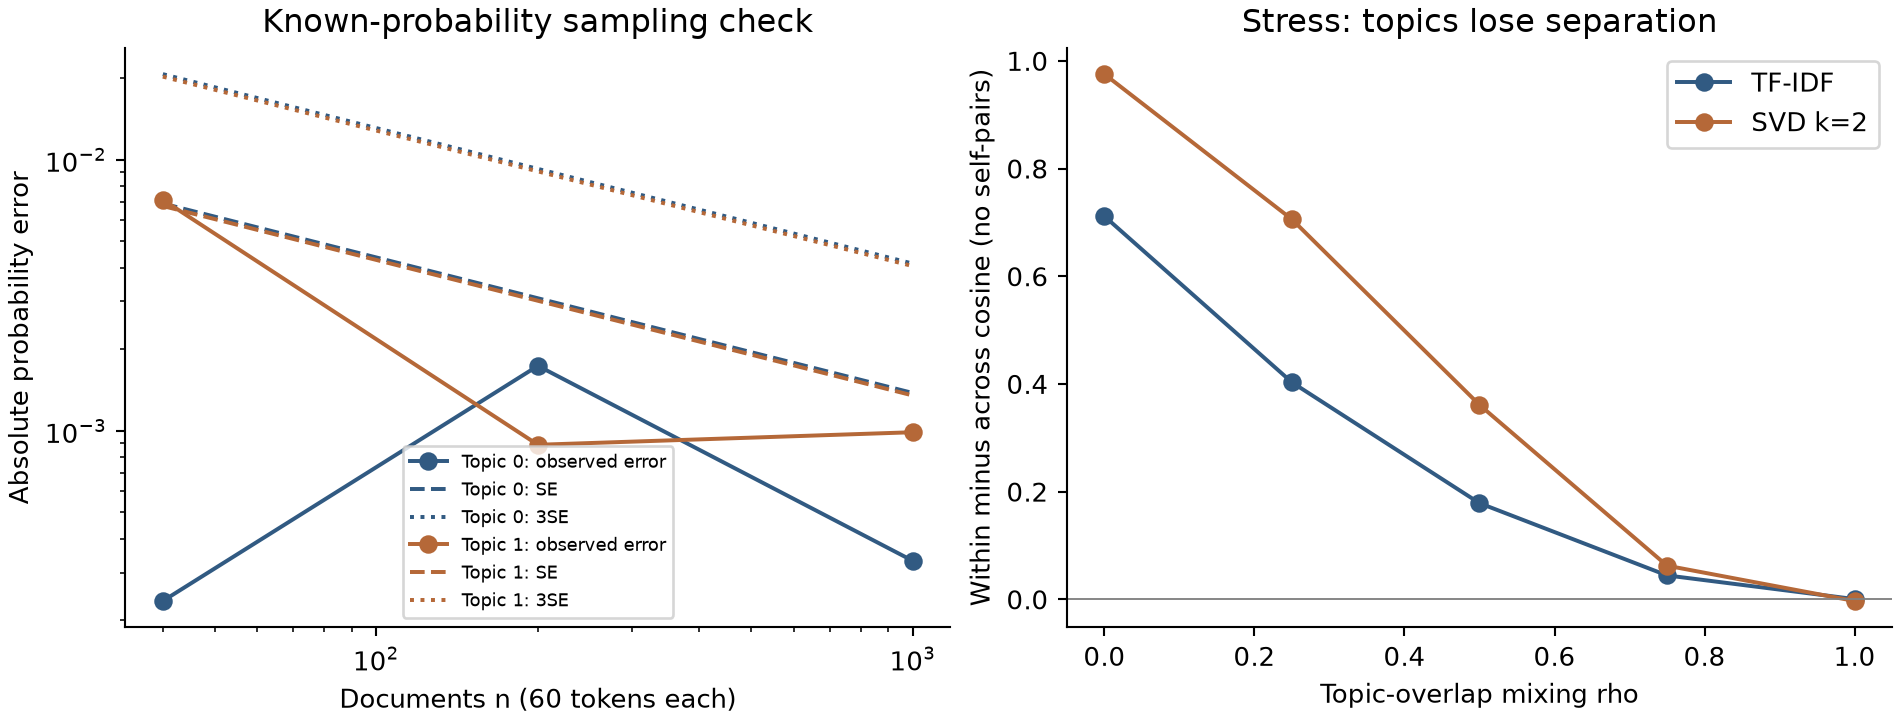
\includegraphics[width=\textwidth]{simulation_checks.png}
\caption{Known-probability error on log-log axes and the topic-overlap stress test.
SE curves are conditional on the fixed drawn topic probabilities.}\end{figure}

\subsection{Stress test: remove topic separation}
The intentional model change is
\[
\theta_h(\rho)=(1-\rho)\theta_h+
\rho(\theta_0+\theta_1)/2,\qquad
\rho\in\{0,0.25,0.5,0.75,1\}.
\]
Seed 0, $n=40$ and 60 tokens per document are retained.
At $\rho=1$, the two distributions coincide and the labels no longer
encode a distributional difference. This breaks the useful-separation
condition, not the algebraic SVD identities.
\input{\resultspath/stress.tex}
The cosine gap closes and the reduced nearest-topic rate falls.
The slightly negative final reduced gap is a finite-sample outcome.
Across-topic similarity can become large even though the numerical
library checks still pass. This is the expected limitation of the
method when topics no longer have distinguishable term distributions.

\section{Real data, cleaning and reproducibility}
The data are the same THUCNews title/body documents from the pinned
Tongjilibo mirror revision
\texttt{ae77e363396e90b54cdaa9eafdbc5e102a3d4019}.
The source prefixes each contain 1,000 records from sports, education
and technology. The original procedure retains at least 30 Chinese
characters, removes exact duplicates within each category, and samples
100 eligible documents per category with seed 0.
The new code uses the recorded IDs rather than selecting a new sample.
\input{\resultspath/cleaning.tex}
The selected title/body strings agree exactly with the local Iteration 2
document table; the character TF-IDF matrix also agrees entry for entry.
No selected document is removed in Iteration 3.
Per-document counts of discarded characters, punctuation and digits
are saved in \path{real_cleaning.csv}. Ordered character and word
token sequences are saved locally as JSONL, with dictionary/settings
and SHA-256 hashes in \texttt{tokenization.json}.
No raw corpus or full processed text is added to Git.

There is no train/test split: this experiment describes similarities
within the fixed collection and uses one of those documents as a
query. Topic labels do not enter counts, IDF or SVD. A future held-out
study would fit vocabulary/IDF using training documents only.
The finite-prefix candidate pool limits representativeness, so these
results do not establish performance on the complete THUCNews corpus.

For TF-IDF verification, scikit-learn's unsmoothed IDF still adds one.
The comparison subtracts that one before applying raw counts and
disables normalization. Comparing against default library TF-IDF
would test a different formula. SVD signs are canonicalized for
readability; reconstruction and cosine comparisons avoid sign ambiguity.
Repeated singular values require subspace comparisons rather than
entrywise equality of arbitrary eigenvectors.

\section{Assumption checks and limitations}
The numerical and frozen-vocabulary checks run on simulation first,
then real data. All recorded known queries match their fitted document
column; adding an OOV token changes no supported coordinate; a fully
unsupported query is rejected. Zero-vector cosine is never assigned
an artificial value.
\input{\resultspath/numerical_assumptions.tex}

\begin{longtable}{p{.25\textwidth}p{.65\textwidth}}
\toprule Assumption / choice & Check and interpretation\\\midrule\endhead
One vocabulary and IDF & Known/mixed-OOV/unsupported query checks pass on all
three simulated sizes and both real representations. Each tokenizer has its
own fixed feature space.\\
Nonzero original and projected vectors & Counts are recorded for both spaces.
No zero real vectors occur. Unsupported queries and explicit zero-vector
test cases raise errors.\\
Positive resolved singular values & Retained values are positive, the energy
rank agrees with a full library spectrum, and boundary ratios are reported.
A looser tolerance $10^{-13}$ changes real cosine matrices by less than
$10^{-8}$. The cutoff is a numerical policy, not proof that excluded
directions have no information.\\
Approximately orthonormal factors & U/V orthogonality, original-Gram residuals,
projection identities and reconstructed-vector cosines are measured.
The normalized Frobenius tail-identity errors pass the stated tolerance.\\
Labels as an imperfect similarity proxy & Known simulation topics give a
controlled reference. Real category means and query inspection disagree
with an unconditional improvement claim. Topic agreement is not semantic
equivalence.\\
No selected exact duplicates & Both representations have zero exact duplicates.
The highest original-cosine pairs are saved for inspection. The leading
character pair, \texttt{technology:685/686}, concerns two reports of a
failed satellite launch; related reporting can inflate neighbor scores
without being exact duplicate text. No such document is silently dropped.\\
Finite-prefix representativeness & The source manifest and original selection
procedure are preserved. No numerical test can make a prefix sample
representative of the whole corpus. The conclusion is restricted to this
fixed collection.\\
Conditional simulated-token independence & Frequencies fall within the displayed
3SE diagnostic. Independence follows from the generator, and cannot be
proved from a finite frequency check. Real text is not assumed to consist
of independent tokens.\\
\bottomrule
\end{longtable}
Bag representations discard order, syntax and compositional meaning.
Simplified/traditional variants are not merged.
Raw counts let longer documents and repeated names influence the SVD.
No stopword filtering was introduced for this comparison.
The larger word vocabulary also contains rare segmentation/name tokens.
These are substantive representation limitations even when every
numerical check passes.

\section{Unified numerical verification}
\path{verification_helpers.py} prints one consistent format and saves
max absolute differences, Frobenius relative differences, tolerance and
pass status. If a reference norm is zero, a nonzero relative difference
is left undefined rather than divided by zero.
Singular-value and cosine comparisons use an absolute $10^{-8}$ limit.
Rank-$k$ reconstruction and the tail identity are compared using
explicitly normalized errors with a $10^{-10}$ limit, avoiding a
scale-dependent test on large squared energies. No raw singular-vector
comparison assumes identical signs.

All \VerificationCount{} deterministic comparison records pass.
Additional tall, wide, rank-deficient, repeated-value, zero-input,
invalid-rank and nonconvergence cases are checked in
\path{verify_iteration3.py}. The following table includes key checks
and the separate sampling comparisons; the full records are in
\path{docs/iteration3/results/verification_all.csv}.
Every displayed difference is generated by a script.
\input{\resultspath/verification.tex}
